\documentclass{article}
\usepackage{enumerate}
\usepackage{amsmath}
\usepackage{amssymb}
\usepackage{graphicx}
\usepackage{subfigure}
\usepackage{geometry}
\usepackage{caption}
\usepackage{indentfirst}
\usepackage{tikz}
\usetikzlibrary{circuits.logic.US}
\usetikzlibrary{arrows.meta}
\usetikzlibrary{calc}
\geometry{left=3.0cm,right=3.0cm,top=3.0cm,bottom=3.0cm}
\renewcommand{\thesection}{Problem \arabic{section}.}
\title{VE270 Homework 7}
\author{Liu Yihao 515370910207}
\date{}

\newcommand{\drawmuxtwo}[3]{
	\draw #1 node (#2) [shape=rectangle,draw,minimum height=2cm,minimum width=2cm,text width=1cm,align=center] {#3};
	\draw (#2) ++(down:7.5mm) node {$s_0$};
	\draw (#2) ++(right:7.5mm) node {$d$};
	\draw (#2) ++(left:7.5mm) ++(up:2.5mm) node {$i_0$} ++(down:5mm) node {$i_1$};
}
\newcommand{\drawmuxfour}[3]{
	\draw #1 node (#2) [shape=rectangle,draw,minimum height=3cm,minimum width=2cm,text width=1cm,align=center] {#3};
	\draw (#2) ++(left:7.5mm) ++(up:7.5mm) node {$i_0$} ++(down:5mm) node {$i_1$} ++(down:5mm) node {$i_2$} ++(down:5mm) node {$i_3$};
	\draw (#2) ++(down:12.5mm)++(left:3.33mm) node {$s_1$} ++(right:6.66mm) node {$s_0$};
	\draw (#2) ++(right:7.5mm) node {$d$};
}
\newcommand{\drawmuxeight}[3]{
	\draw #1 node (#2) [shape=rectangle,draw,minimum height=5cm,minimum width=2cm,text width=1cm,align=center] {#3};
	\draw (#2) ++(left:7.5mm) ++(up:17.5mm) node {$i_0$} ++(down:5mm) node {$i_1$} ++(down:5mm) node {$i_2$} ++(down:5mm) node {$i_3$} ++(down:5mm) node {$i_4$} ++(down:5mm) node {$i_5$} ++(down:5mm) node {$i_6$} ++(down:5mm) node {$i_7$};
	\draw (#2) ++(down:22.5mm) node {$s_1$} ++(left:5mm) node {$s_2$} ++(right:10mm) node {$s_0$};
	\draw (#2) ++(right:7.5mm) node {$d$};
}
\newcommand{\drawdecodereight}[3]{
	\draw #1 node (#2) [shape=rectangle,draw,minimum height=5cm,minimum width=2cm,text width=1cm,align=center] {#3};
	\draw (#2) ++(right:7.5mm) ++(up:17.5mm) node {$d_0$} ++(down:5mm) node {$d_1$} ++(down:5mm) node {$d_2$} ++(down:5mm) node {$d_3$} ++(down:5mm) node {$d_4$} ++(down:5mm) node {$d_5$} ++(down:5mm) node {$d_6$} ++(down:5mm) node {$d_7$};
	\draw (#2) ++(left:7.5mm) node {$i_1$} ++(up:5mm) node {$i_0$} ++(down:10mm) node {$i_2$};
}

\begin{document}
\maketitle

\section{}
\begin{center}
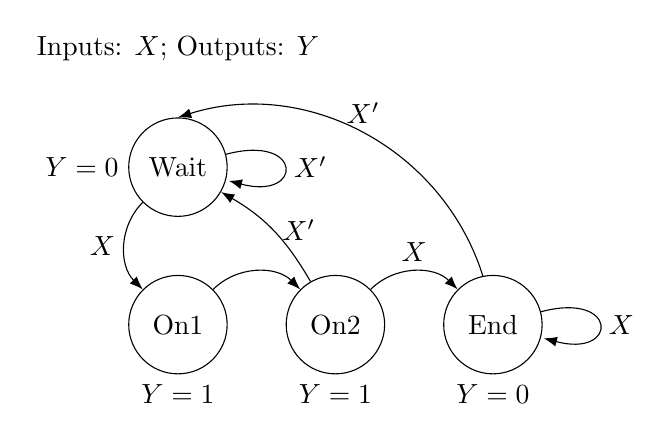
\begin{tikzpicture}[>/.tip={Latex}]
	\draw (0,0.5) node (io) {Inputs: $X$; Outputs: $Y$};
	\draw (0,-1) node (wait) [draw,shape=circle,minimum size=1.25cm] {Wait};
	\node [left] at (wait.west) {$Y=0$};
	\draw (0,-3) node (on1) [draw,shape=circle,minimum size=1.25cm] {On1};
	\node [below] at (on1.south) {$Y=1$};
	\draw (2,-3) node (on2) [draw,shape=circle,minimum size=1.25cm] {On2};
	\node [below] at (on2.south) {$Y=1$};
	\draw (4,-3) node (end) [draw,shape=circle,minimum size=1.25cm] {End};
	\node [below] at (end.south) {$Y=0$};

	\draw[->] (wait) edge [loop right] node {$X'$} ();
	\draw[->] (wait) edge [bend right=45] node [left] {$X$} (on1);
	\draw[->] (on1) edge [bend left=45] node {} (on2);
	\draw[->] (on2) edge [bend left=45] node [above] {$X$} (end);
	\draw[->] (on2) [bend right=15] edge node [right] {$X'$} (wait);
	\draw[->] (end) edge [loop right] node {$X$} ();
	\draw[->] (end) edge [bend right=45] node [above] {$X'$} (wait.north);
\end{tikzpicture}
\end{center}

\section{}
Encode the states ($s_1s_0$): Wait: 00, On1: 10, On2: 11, End: 01.

\begin{center}
\begin{tikzpicture}
	\drawfsmreigistertwo{(0,0)}{r}{2-bit state register}{2};
	\draw (r.west) ++(left:1.5cm) node (clock) {clock};
	\draw (r.west) -- (clock);
	\draw (r.south) ++(left:5mm) -- ++(down:2cm) -- ++(right:1.5cm) node (s1){};
	\draw (r.south) ++(right:5mm)-- ++(down:2.5cm) --  ++(right:1.5cm) node (s0){};
	\draw (s1) ++(right:7cm) node (Y) {Y};
	\draw (Y) -- ++(left:7cm);
	\drawfsmmuxtwo{(r)++(right:6cm)}{m}{2-bit 4x2 mux};
	\filldraw (m.south) ++(left:3.3mm) ++(down:0.5cm) circle [radius=0.5mm];
	\draw (m.south) ++(left:3.3mm) -- ++(down:0.5cm);
	\draw (m.south) ++(right:3.3mm) |- (s0.west);	
	\draw (m.east) ++(up:2.5mm) -- ++(right:1cm) -- ++(up:3.25cm) -| ($(r.north)+(left:5mm)$);
	\draw (m.east) ++(down:2.5mm) -- ++(right:1.5cm) -- ++(up:3.25cm) -| ($(r.north)+(right:5mm)$);
	\draw (m.west) ++(up:17.5mm) ++(left:4cm) node (X) {$X$};
	\draw (m.west) ++(up:12.5mm) ++(left:1cm) node (b0) {0};
	\draw (m.west) ++(up:7.5mm) ++(left:1cm) node (a1) {0};
	\draw (m.west) ++(down:2.5mm) ++(left:1cm) node (a2) {1};
	\draw (m.west) ++(down:7.5mm) ++(left:1cm) node (b2) {1};
	\draw (m.west) ++(down:12.5mm) ++(left:1cm) node (a3) {1};
	\draw (b0) -- ++(right:1cm) (a1) -- ++(right:1cm) (a2) -- ++(right:1cm) (b2) -- ++(right:1cm) (a3) -- ++(right:1cm);
	\draw (X) -- ++(right:4cm);
	\draw (X) ++(right:1cm) |- ($(m.west)+(down:17.5mm)$);
	\draw (X) ++(right:1cm) |- ($(m.west)+(up:2.5mm)$);
	\filldraw (X) ++(right:1cm) circle [radius=0.5mm] ++(down:1.5cm) circle [radius=0.5mm];
\end{tikzpicture}
\end{center}



\section{}
\begin{center}
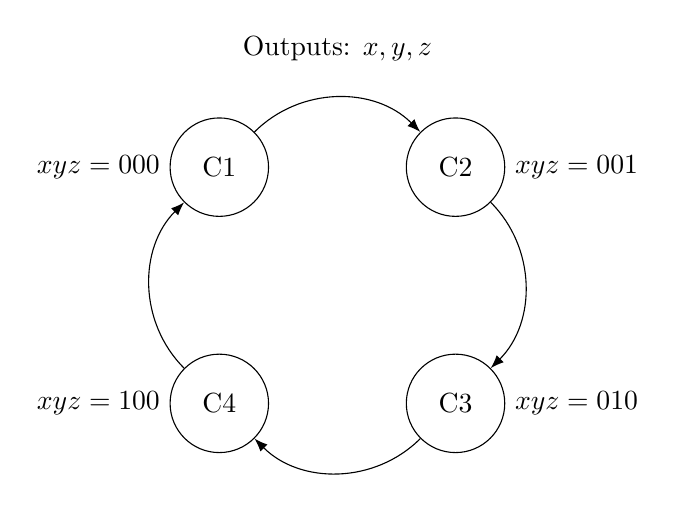
\begin{tikzpicture}[>/.tip={Latex}]
	\draw (0,3) node (io) {Outputs: $x,y,z$};
	\draw (-1.5,1.5) node(C1) [draw,shape=circle,minimum size=1.25cm] {C1};
	\node [left] at (C1.west) {$xyz=000$};
	\draw (1.5,1.5) node(C2) [draw,shape=circle,minimum size=1.25cm] {C2};
	\node [right] at (C2.east) {$xyz=001$};
	\draw (1.5,-1.5) node(C3) [draw,shape=circle,minimum size=1.25cm] {C3};
	\node [right] at (C3.east) {$xyz=010$};
	\draw (-1.5,-1.5) node(C4) [draw,shape=circle,minimum size=1.25cm] {C4};
	\node [left] at (C4.west) {$xyz=100$};
	\draw[->] (C1) edge [bend left=45] (C2);
	\draw[->] (C2) edge [bend left=45] (C3);
	\draw[->] (C3) edge [bend left=45] (C4);
	\draw[->] (C4) edge [bend left=45] (C1);
\end{tikzpicture}
\end{center}

\section{}
\begin{center}
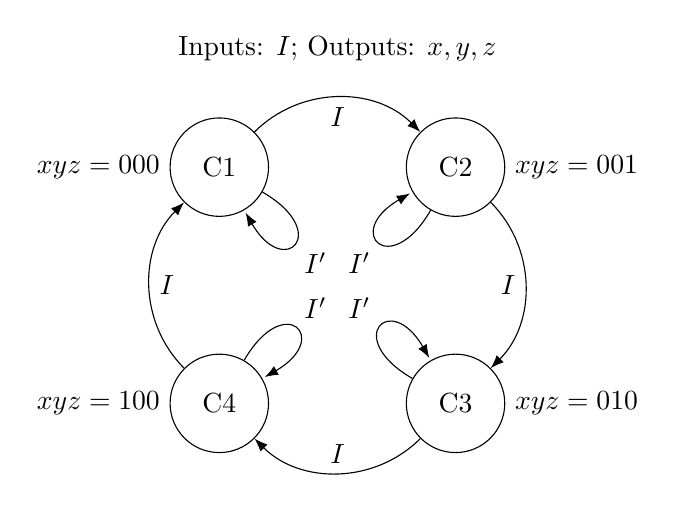
\begin{tikzpicture}[>/.tip={Latex}]
	\draw (0,3) node (io) {Inputs: $I$; Outputs: $x,y,z$};
	\draw (-1.5,1.5) node(C1) [draw,shape=circle,minimum size=1.25cm] {C1};
	\node [left] at (C1.west) {$xyz=000$};
	\draw (1.5,1.5) node(C2) [draw,shape=circle,minimum size=1.25cm] {C2};
	\node [right] at (C2.east) {$xyz=001$};
	\draw (1.5,-1.5) node(C3) [draw,shape=circle,minimum size=1.25cm] {C3};
	\node [right] at (C3.east) {$xyz=010$};
	\draw (-1.5,-1.5) node(C4) [draw,shape=circle,minimum size=1.25cm] {C4};
	\node [left] at (C4.west) {$xyz=100$};
	\draw[->] (C1) edge [bend left=45] node [below] {$I$} (C2);
	\draw[->] (C2) edge [bend left=45] node [left] {$I$} (C3);
	\draw[->] (C3) edge [bend left=45] node [above] {$I$} (C4);
	\draw[->] (C4) edge [bend left=45] node [right] {$I$} (C1);
	\draw[->] (C1) edge [in=300,out=330,loop] node [below right] {$I'$} ();
	\draw[->] (C2) edge [in=210,out=240,loop] node [below left] {$I'$} ();
	\draw[->] (C3) edge [in=120,out=150,loop] node [above left] {$I'$} ();
	\draw[->] (C4) edge [in=30,out=60,loop] node [above right] {$I'$} ();
\end{tikzpicture}
\end{center}

\section{}
\begin{center}
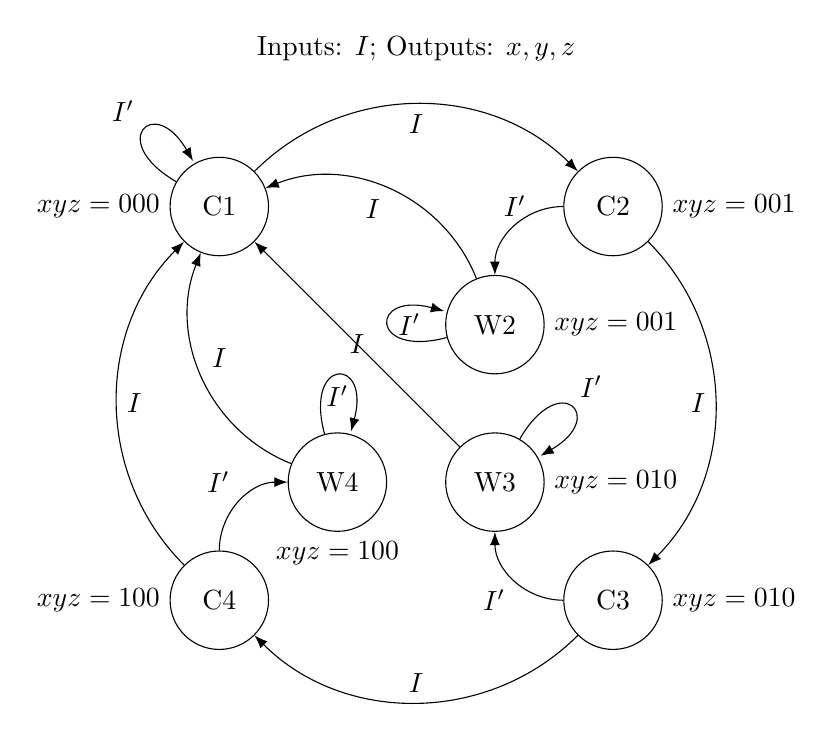
\begin{tikzpicture}[>/.tip={Latex}]
	\draw (0,4.5) node (io) {Inputs: $I$; Outputs: $x,y,z$};
	\draw (-2.5,2.5) node(C1) [draw,shape=circle,minimum size=1.25cm] {C1};
	\node [left] at (C1.west) {$xyz=000$};
	\draw (2.5,2.5) node(C2) [draw,shape=circle,minimum size=1.25cm] {C2};
	\node [right] at (C2.east) {$xyz=001$};
	\draw (1,1) node(W2) [draw,shape=circle,minimum size=1.25cm] {W2};
	\node [right] at (W2.east) {$xyz=001$};
	\draw (2.5,-2.5) node(C3) [draw,shape=circle,minimum size=1.25cm] {C3};
	\node [right] at (C3.east) {$xyz=010$};
	\draw (1,-1) node(W3) [draw,shape=circle,minimum size=1.25cm] {W3};
	\node [right] at (W3.east) {$xyz=010$};
	\draw (-2.5,-2.5) node(C4) [draw,shape=circle,minimum size=1.25cm] {C4};
	\node [left] at (C4.west) {$xyz=100$};
	\draw (-1,-1) node(W4) [draw,shape=circle,minimum size=1.25cm] {W4};
	\node [below] at (W4.south) {$xyz=100$};
	\draw[->] (C1) edge [bend left=45] node [below] {$I$} (C2);
	\draw[->] (C2) edge [bend left=45] node [left] {$I$} (C3);
	\draw[->] (C3) edge [bend left=45] node [above] {$I$} (C4);
	\draw[->] (C4) edge [bend left=45] node [right] {$I$} (C1);
	\draw[->] (C1) edge [in=120,out=150,loop] node [above left] {$I'$} ();
	\draw[->] (C2) edge [bend right=45] node [above] {$I'$} (W2);
	\draw[->] (W2) edge [bend right=45] node [below left] {$I$} (C1);
	\draw[->] (C3) edge [bend left=45] node [below left] {$I'$} (W3);
	\draw[->] (W3) edge node {$I$} (C1);
	\draw[->] (C4) edge [bend left=45] node [above left] {$I'$} (W4);
	\draw[->] (W4) edge [bend left=45] node [above right] {$I$} (C1);
	\draw[->] (W2) edge [loop left] node [right] {$I'$} ();
	\draw[->] (W3) edge [in=30,out=60,loop] node [above right] {$I'$} ();
	\draw[->] (W4) edge [loop above] node [below] {$I'$} ();
\end{tikzpicture}
\end{center}

\section{}

Encode the states ($s_1s_0$): Wait: 00, On1: 10, On2: 11, End: 01.

\begin{center}
\begin{tikzpicture}
	\drawfsmreigistertwo{(0,0)}{r}{2-bit state register}{2};
	\draw (r.west) ++(left:1.5cm) node (clock) {clock};
	\draw (r.west) -- (clock);
	\draw (r.south) ++(left:5mm) -- ++(down:2cm) -- ++(right:1.5cm) node (s1){};
	\draw (r.south) ++(right:5mm)-- ++(down:2.5cm) --  ++(right:1.5cm) node (s0){};
	\draw (s1) ++(right:7cm) node (Y) {Y};
	\draw (Y) -- ++(left:7cm);
	\drawfsmmuxtwo{(r)++(right:6cm)}{m}{2-bit 4x2 mux};
	\filldraw (m.south) ++(left:3.3mm) ++(down:0.5cm) circle [radius=0.5mm];
	\draw (m.south) ++(left:3.3mm) -- ++(down:0.5cm);
	\draw (m.south) ++(right:3.3mm) |- (s0.west);	
	\draw (m.east) ++(up:2.5mm) -- ++(right:1cm) -- ++(up:3.25cm) -| ($(r.north)+(left:5mm)$);
	\draw (m.east) ++(down:2.5mm) -- ++(right:1.5cm) -- ++(up:3.25cm) -| ($(r.north)+(right:5mm)$);
	\draw (m.west) ++(up:17.5mm) ++(left:4cm) node (X) {$X$};
	\draw (m.west) ++(up:12.5mm) ++(left:1cm) node (b0) {0};
	\draw (m.west) ++(up:7.5mm) ++(left:1cm) node (a1) {0};
	\draw (m.west) ++(down:2.5mm) ++(left:1cm) node (a2) {1};
	\draw (m.west) ++(down:7.5mm) ++(left:1cm) node (b2) {1};
	\draw (m.west) ++(down:12.5mm) ++(left:1cm) node (a3) {1};
	\draw (b0) -- ++(right:1cm) (a1) -- ++(right:1cm) (a2) -- ++(right:1cm) (b2) -- ++(right:1cm) (a3) -- ++(right:1cm);
	\draw (X) -- ++(right:4cm);
	\draw (X) ++(right:1cm) |- ($(m.west)+(down:17.5mm)$);
	\draw (X) ++(right:1cm) |- ($(m.west)+(up:2.5mm)$);
	\filldraw (X) ++(right:1cm) circle [radius=0.5mm] ++(down:1.5cm) circle [radius=0.5mm];
\end{tikzpicture}
\end{center}


\section{}
\begin{center}
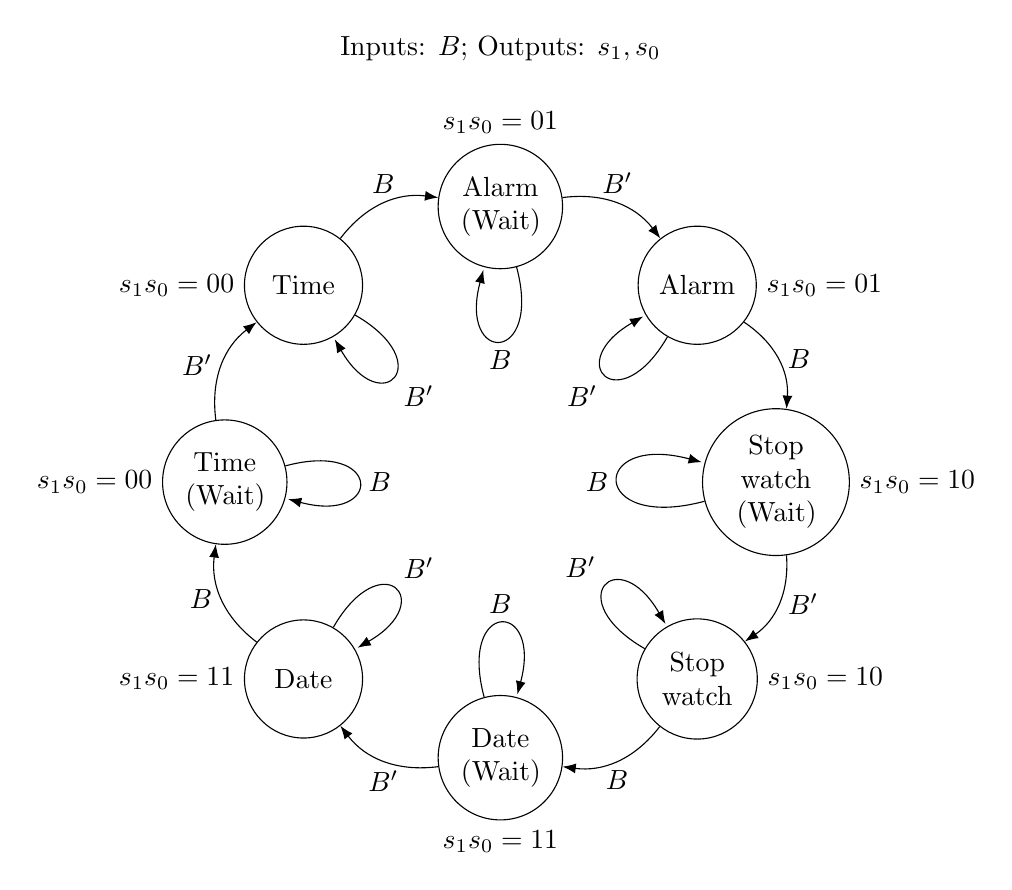
\begin{tikzpicture}[>/.tip={Latex}]
	\draw (0,5.5) node (io) {Inputs: $B$; Outputs: $s_1,s_0$};
	\draw (-2.5,2.5) node (C1) [draw,shape=circle,minimum size=1.5cm,text width=1cm,align=center] {Time};
	\node [left] at (C1.west) {$s_1s_0=00$};
	\draw (0,3.5) node (W2) [draw,shape=circle,minimum size=1.5cm,text width=1cm,align=center] {Alarm (Wait)};
	\node [above] at (W2.north) {$s_1s_0=01$};
	\draw (2.5,2.5) node (C2) [draw,shape=circle,minimum size=1.5cm,text width=1cm,align=center] {Alarm};
	\node [right] at (C2.east) {$s_1s_0=01$};
	\draw (3.5,0) node (W3) [draw,shape=circle,minimum size=1.5cm,text width=1cm,align=center] {Stop watch (Wait)};
	\node [right] at (W3.east) {$s_1s_0=10$};
	\draw (2.5,-2.5) node (C3) [draw,shape=circle,minimum size=1.5cm,text width=1cm,align=center] {Stop watch};
	\node [right] at (C3.east) {$s_1s_0=10$};
	\draw (0,-3.5) node (W4) [draw,shape=circle,minimum size=1.5cm,text width=1cm,align=center] {Date (Wait)};
	\node [below] at (W4.south) {$s_1s_0=11$};
	\draw (-2.5,-2.5) node (C4) [draw,shape=circle,minimum size=1.5cm,text width=1cm,align=center] {Date};
	\node [left] at (C4.west) {$s_1s_0=11$};
	\draw (-3.5,0) node (W1) [draw,shape=circle,minimum size=1.5cm,text width=1cm,align=center] {Time (Wait)};
	\node [left] at (W1.west) {$s_1s_0=00$};
	\draw[->] (C1) edge [bend left=30] node [above] {$B$} (W2);
	\draw[->] (W2) edge [bend left=30] node [above] {$B'$} (C2);
	\draw[->] (C2) edge [bend left=30] node [right] {$B$} (W3);
	\draw[->] (W3) edge [bend left=30] node [right] {$B'$} (C3);
	\draw[->] (C3) edge [bend left=30] node [below] {$B$} (W4);
	\draw[->] (W4) edge [bend left=30] node [below] {$B'$} (C4);
	\draw[->] (C4) edge [bend left=30] node [left] {$B$} (W1);
	\draw[->] (W1) edge [bend left=30] node [left] {$B'$} (C1);
	\draw[->] (C1) edge [in=300,out=330,loop] node [below right] {$B'$} ();
	\draw[->] (W2) edge [loop below] node [below] {$B$} ();
	\draw[->] (C2) edge [in=210,out=240,loop] node [below left] {$B'$} ();
	\draw[->] (W3) edge [loop left] node [left] {$B$} ();
	\draw[->] (C3) edge [in=120,out=150,loop] node [above left] {$B'$} ();
	\draw[->] (W4) edge [loop above] node [above] {$B$} ();
	\draw[->] (C4) edge [in=30,out=60,loop] node [above right] {$B'$} ();
	\draw[->] (W1) edge [loop right] node [right] {$B$} ();
\end{tikzpicture}
\end{center}


\end{document}
